\documentclass[aspectratio=169,11pt]{beamer}

\usepackage[utf8]{inputenc}
\usepackage[T1]{fontenc}
\usepackage{lmodern}
\usepackage{amsmath,amssymb}
\usepackage{booktabs}
\usepackage{graphicx}
\usepackage{xcolor}
\usepackage{tcolorbox}

% --- Theme: clean default ---
\usetheme{default}
\usecolortheme{seahorse}
\setbeamertemplate{navigation symbols}{}
\setbeamertemplate{footline}[frame number]
\setbeamertemplate{itemize items}[circle]
\setbeamerfont{title}{size=\Large,series=\bfseries}
\setbeamerfont{frametitle}{size=\large,series=\bfseries}
\setbeamerfont{framesubtitle}{size=\small,shape=\itshape}
\setbeamercolor{title}{fg=structure!85!black}
\setbeamercolor{frametitle}{fg=structure!85!black}

% --- Custom commands ---
\definecolor{accent}{HTML}{1F77B4}
\definecolor{warm}{HTML}{D95F02}
\definecolor{ok}{HTML}{1B9E77}
\newcommand{\hilite}[1]{\textcolor{accent}{\textbf{#1}}}
\newcommand{\warn}[1]{\textcolor{warm}{\textbf{#1}}}
\newcommand{\good}[1]{\textcolor{ok}{\textbf{#1}}}

\newtcolorbox{sigbox}{
  colback=gray!7, colframe=gray!50, boxrule=0.4pt, arc=1pt,
  left=4pt, right=4pt, top=2pt, bottom=2pt, fontupper=\scriptsize\ttfamily}

\title{Quantitative Trading and Price Impact}
\subtitle{End-to-end pipeline with non-parametric impact \\ and multi-day carry backtest}
\author{Anran Severac}
\institute{MSc Mathematics \& Finance \,\textbar\, Final Project}
\date{May 15, 2026}

\begin{document}

% ============================================================
% 1. TITLE
% ============================================================
\begin{frame}[plain]
  \titlepage
  \vspace*{-1em}
  \centering
  \scriptsize\itshape
  Modular \texttt{src/price\_impact/} package \,\textbar\, thin orchestration
  notebook \,\textbar\, every backtest run writes to \texttt{saved/<name>/}
\end{frame}

% ============================================================
% 2. PIPELINE AT A GLANCE
% ============================================================
\begin{frame}{Pipeline at a glance}{Seven assignment sections, eight modules, two enhancements}

  \begin{columns}[T]
  \column{0.52\textwidth}
  \scriptsize
  \textbf{Modules vs assignment sections}
  \begin{tabular}{lll}
  \toprule
  Module & Responsibility & Section \\
  \midrule
  \texttt{data}          & top-$N$, $\sigma$/ADV    & \S2.1 \\
  \texttt{impact\_states}& OU $\bar I$ (daily + multi) & \S2.2/\S2.3 \\
  \texttt{fitting}       & OLS + NP + $H$-grid    & \S2.2 \\
  \texttt{alpha}         & synthetic $\alpha$        & \S2.4 \\
  \texttt{strategy}      & OW/AFS/ext-OW             & \S2.5 \\
  \texttt{backtest}      & Waelbroeck sim            & \S2.3 \\
  \texttt{results}       & metrics + TCA + plots     & \S2.6 \\
  \texttt{runner}        & \texttt{BacktestConfig}$\to$disk & \S2.6/\S2.7 \\
  \bottomrule
  \end{tabular}

  \column{0.46\textwidth}
  \scriptsize
  \textbf{Design principles}
  \begin{itemize}
    \item Single-responsibility modules; notebook is glue
    \item Same simulator runs \hilite{any} signed trade path
    \item Carry mode = one flag; downstream unchanged
    \item Every run dumps tables + plots to \texttt{saved/<name>/}
  \end{itemize}
  \end{columns}

  \vspace{0.6em}
  \begin{center}
  \footnotesize\textbf{Two enhancements emphasised:}\;\;
  \hilite{NP impact} with cross-stock $\gamma$ shrinkage (\S2.2)\;\;$\bullet$\;\;
  \hilite{Multi-day carry} backtest engine (\S2.3)\\[2pt]
  \scriptsize\itshape Solo submission -- all sections by author.
  \end{center}
\end{frame}

% ============================================================
% 3. DATA PREP
% ============================================================
\begin{frame}{Data preparation \hfill \emph{\S2.1 -- baseline}}{2019 panel, 10-second bins, trailing-20-day daily stats}

  \begin{columns}[T]
  \column{0.55\textwidth}
  \footnotesize
  \textbf{Panel}
  \begin{itemize}
    \item 2019 US equities, 10-s bins (monthly CSVs ${\sim}200$\,MB each)
    \item \hilite{Top-20 stocks} by full-year total $|q_t|$
    \item Final panel: $\sim$11.0M bin rows, 250 trading days
  \end{itemize}

  \vspace{0.4em}
  \textbf{Daily statistics} (trailing 20-day rolling)
  \[
    \sigma_{i,d}^2 = \overline{\mathrm{Var}_t r_{i,d,t}},\qquad
    \mathrm{ADV}_{i,d} = \overline{\textstyle\sum_t |q_{i,d,t}|}
  \]
  Used to normalise flow so impact coefficients are comparable across stocks and days.

  \column{0.43\textwidth}
  \footnotesize
  \textbf{In-sample / out-of-sample protocol}\\
  10 rolling windows:
  \begin{itemize}
    \item train on month $m$
    \item tune $\gamma$ on $m{+}1$ (NP only)
    \item validate on $m{+}2$
  \end{itemize}
  for $m = 1,\dots,10$.

  \vspace{0.7em}
  \begin{sigbox}
  build\_panel(data\_dir, year, top\_n=20,\\
  \hspace*{1.5em}lookback\_days=20)\\
  \hspace*{0.5em}$\to$ PanelData(bins, daily\_stats, stocks)
  \end{sigbox}

  \vspace{0.4em}
  \footnotesize\itshape
  Module \texttt{data} = 165 lines, deterministic, no I/O outside the bin CSVs.
  \end{columns}
\end{frame}

% ============================================================
% 4. IMPACT-STATE RECURSION
% ============================================================
\begin{frame}{Impact-state recursion \hfill \emph{\S2.2}}{OW vs AFS, daily-reset vs multi-day $\bar I$}

  \begin{columns}[T]
  \column{0.52\textwidth}
  \footnotesize
  Both models build the OU recursion
  \[
    \bar I_{t+1} = (1-\beta)\bar I_t + \tilde q_t,
    \qquad \beta = \frac{\ln 2}{H_{\text{bins}}}.
  \]
  They differ only in the kernel applied to raw flow:
  \[
    \text{\hilite{OW}:}\;\;\tilde q_t = \sigma\,q_t/\mathrm{ADV}
  \]
  \[
    \text{\hilite{AFS}:}\;\;\tilde q_t = \sigma\,\mathrm{sgn}(q_t)\sqrt{|q_t|/\mathrm{ADV}}
  \]

  \vspace{0.4em}
  \textbf{Two carry modes produced side-by-side}
  \begin{itemize}
    \item \texttt{I\_bar\_daily} -- reset at each session
    \item \texttt{I\_bar\_multi} -- carry with overnight decay $(1-\beta)^{16\text{h}\cdot 6}$
  \end{itemize}

  \column{0.46\textwidth}
  \centering
  
\includegraphics[width=\linewidth]{figures/ibar_daily_vs_multi.png}

  \footnotesize\itshape
  At $H=60$\,min the overnight decay $(1-\beta)^{5760} \approx 10^{-5}$ already wipes $\bar I$, so the two curves overlap on screen. The flag still matters for the backtest because \hilite{inventory} carries even when $\bar I$ does not.
  \end{columns}
\end{frame}

% ============================================================
% 5. HALF-LIFE GRID SEARCH
% ============================================================
\begin{frame}{Half-life grid search \hfill \emph{\S2.2}}{Empirical $H$ via rolling-OOS sweep}

  \begin{columns}[T]
  \column{0.42\textwidth}
  \footnotesize
  9-point grid $H \in \{5,10,20,30,45,60,90,120,180\}$\,min;\\
  for each $(H,\text{model})$ run rolling OLS and average OOS $R^2$.

  \vspace{0.5em}
  \begin{tabular}{lcc}
  \toprule
  $H$ (min) & OW & AFS \\
  \midrule
  30  & 0.1579 & 0.2604 \\
  \textbf{45}  & 0.1582 & \textbf{0.2609} \\
  \textbf{60}  & \textbf{0.1583} & 0.2608 \\
  90  & 0.1581 & 0.2602 \\
  120 & 0.1578 & 0.2595 \\
  \bottomrule
  \end{tabular}

  \vspace{0.4em}
  \good{$H^* = 52.5$ min} (midpoint).\\
  Cost of universal $H^*$ vs per-model optimum: $<10^{-4}$.\\
  AFS dominates OW by \hilite{${\sim}10$\,pp} in OOS $R^2$.

  \column{0.56\textwidth}
  \centering
  \includegraphics[width=\linewidth]{figures/halflife_grid_search.png}
  \end{columns}
\end{frame}

% ============================================================
% 6. NON-PARAMETRIC + GAMMA SHRINKAGE
% ============================================================
\begin{frame}{Non-parametric extension + $\gamma$ shrinkage \hfill \warn{ENHANCEMENT \#1}}{Three-sample protocol; method recap}

  \begin{columns}[T]
  \column{0.46\textwidth}
  \footnotesize
  Replace $y = \alpha + \lambda x$ with a binned $g(x)$:
  \[
    g_{i,b}^{\mathrm{reg}}(\gamma)
    = \frac{S_{y,i,b} + \gamma\,\bar g_b}{n_{i,b}+\gamma}
  \]
  \begin{itemize}
    \item $B=15$ quantile bins on train month $m$ (pooled across stocks)
    \item $\bar g_b$ = pooled universal curve
    \item \hilite{$\gamma$ tuned on test month $m{+}1$} (MSE), validated on $m{+}2$
  \end{itemize}

  \vspace{0.3em}
  \textbf{Why three samples?}\\
  Tuning $\gamma$ on the validation month leaks. We need
  \emph{train, tune, validate} -- distinct months, in order.

  \vspace{0.4em}
  \begin{sigbox}
  rolling\_nonparametric(features,\\
  \hspace*{1.5em}n\_bins=15, n\_windows=10)\\
  \hspace*{0.5em}$\to$ (summary DF, fits dict)
  \end{sigbox}

  \column{0.52\textwidth}
  \centering
  \includegraphics[width=\linewidth]{figures/gamma_tuning_curves.png}

  \footnotesize\itshape
  Tuning curves flat across 6 orders of magnitude $\Rightarrow$ in the headline configuration (median $n \approx 3000$ per (stock, bin)) the per-stock estimator is already precise; shrinkage has nothing to fix. We'll see in \emph{slide 12} that the estimator behaves correctly when it does need to fix something.
  \end{columns}
\end{frame}

% ============================================================
% 7. HEADLINE OOS R²
% ============================================================
\begin{frame}{Headline OOS $R^2$ \hfill \emph{\S2.2}}{Apples-to-apples comparison + estimated impact curves}

  \begin{columns}[T]
  \column{0.46\textwidth}
  \footnotesize
  \textbf{Pooled OOS $R^2$ (panel-wide null, same merged subset)}

  \vspace{0.3em}
  \begin{tabular}{lccc}
  \toprule
  Model & Param. & NP Reg. & $\Delta$ \\
  \midrule
  OW  & 0.1612 & \good{0.2206} & \good{$+0.059$} \\
  AFS & 0.2689 & 0.2629 & $-0.006$ \\
  \bottomrule
  \end{tabular}

  \vspace{0.6em}
  \textbf{Two findings}
  \begin{itemize}
    \item \hilite{NP lifts OW by $+5.9$\,pp} -- linearity is a binding constraint
    \item \hilite{NP ties AFS} ($-0.6$\,pp): the 1-parameter sqrt form sits on the efficient frontier; 15 parameters buy nothing
  \end{itemize}

  \vspace{0.3em}
  \footnotesize\itshape
  Aggregation matters: under per-stock $R^2$ averaging, NP appears to beat AFS by $+0.2$\,pp -- an artefact that disappears under pooled $R^2$.

  \column{0.52\textwidth}
  \centering
  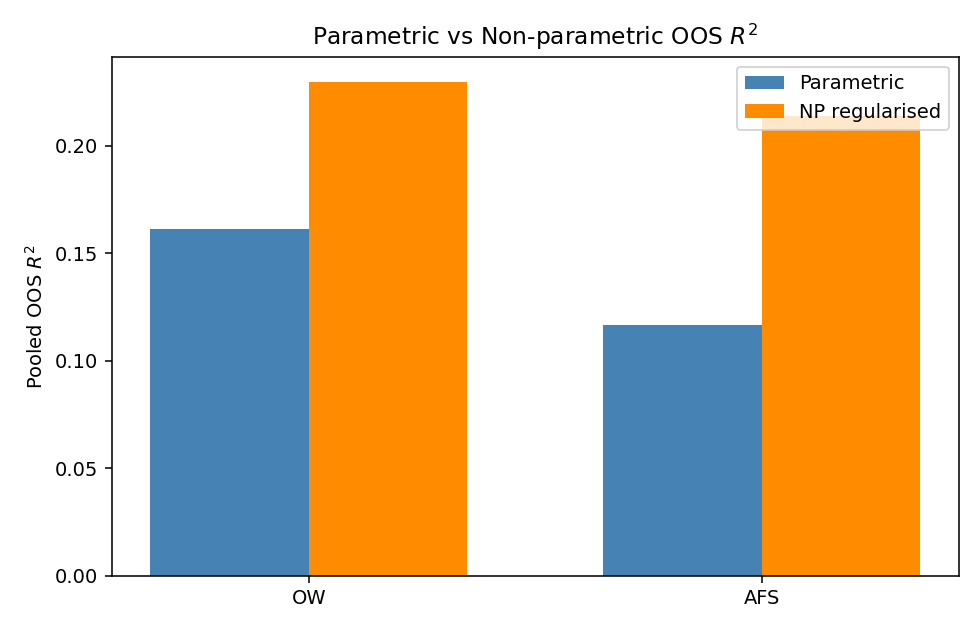
\includegraphics[width=0.92\linewidth]{figures/parametric_vs_nonparametric.png}\\[2pt]
  {\scriptsize OOS $R^2$: parametric OLS vs NP estimators}

  \vspace{0.5em}
  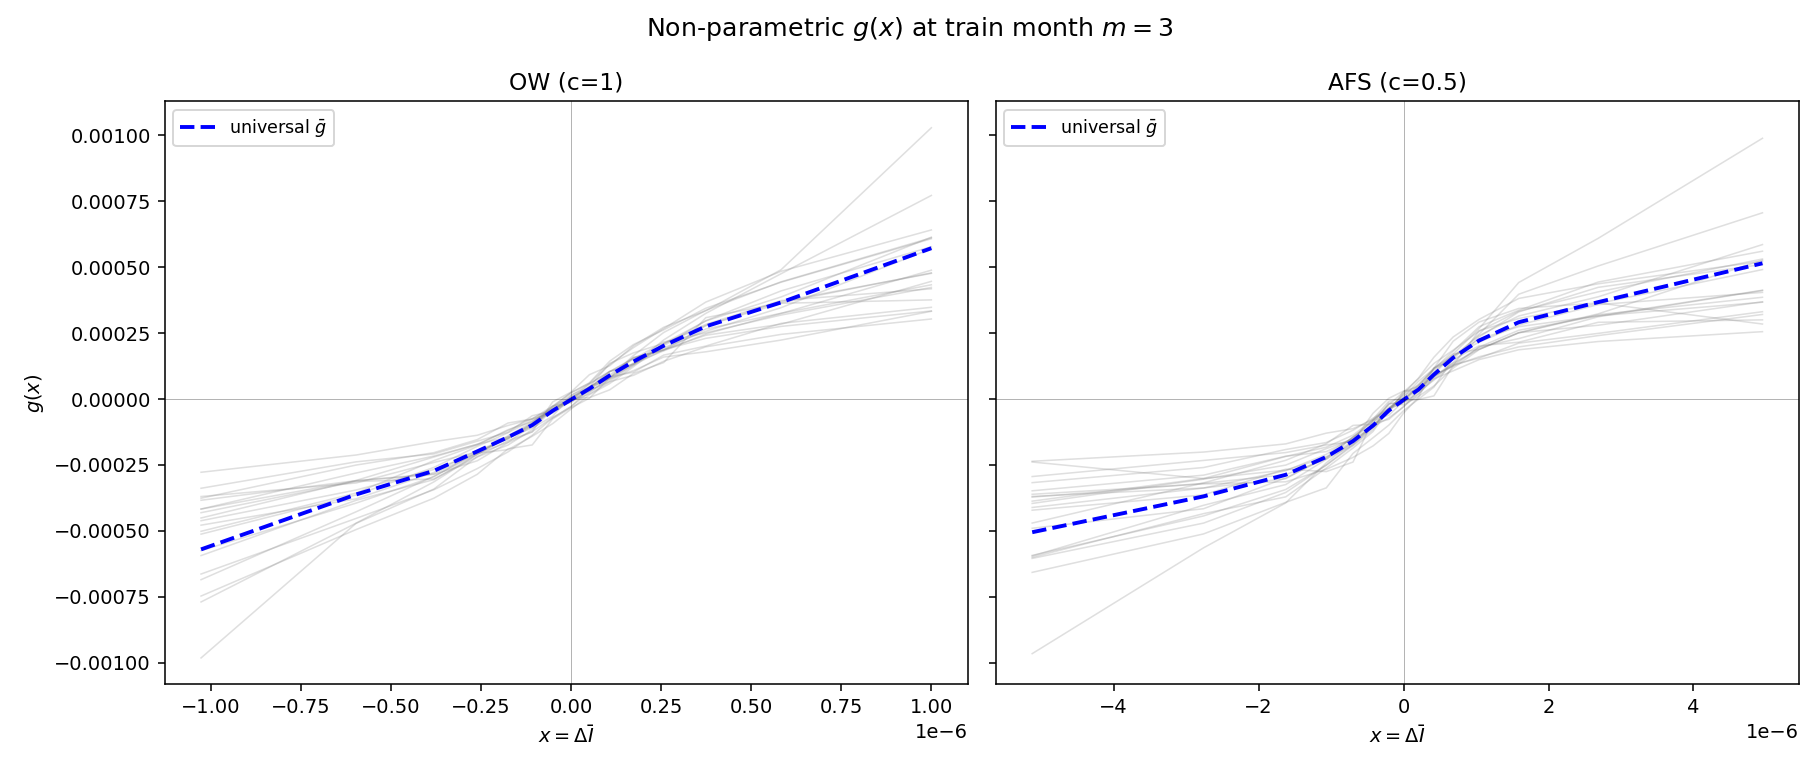
\includegraphics[width=0.92\linewidth]{figures/impact_curves.png}\\[2pt]
  {\scriptsize\itshape Per-stock $\hat g_i$ (grey) cluster tightly around universal $\bar g$ (dashed); AFS shows concavity.}
  \end{columns}
\end{frame}

% ============================================================
% 8. BACKTEST ENGINE
% ============================================================
\begin{frame}{Backtest engine \hfill \warn{\S2.3 -- ENHANCEMENT \#2}}{Waelbroeck + carry modes + generic-trade interface}

  \[
    P_{\text{sim}}(t) = P_0\bigl(1 + \mathrm{cumret}(t) + g_{\text{sim}}(t) - g_{\text{ref}}(t)\bigr),
    \quad g(t) = \lambda\,\bar I(t)\;\;\text{or}\;\;\lambda(t)\,\bar I(t)
  \]
  $\bar I^{\text{ref}}$ uses public-tape \texttt{orderFlow}; $\bar I^{\text{sim}}$ uses the simulator's input trade path.

  \begin{columns}[T]
  \column{0.5\textwidth}
  \footnotesize
  \textbf{Generic trades.}
  Engine accepts any signed schedule via a \texttt{trade\_provider} callable:
  \begin{itemize}
    \item \texttt{make\_optimal\_provider(strategy\_fn)} -- OW/AFS
    \item \texttt{make\_fixed\_provider(trades)} -- TWAP/VWAP/manual
  \end{itemize}
  \textbf{Carry modes.}
  \begin{itemize}
    \item \texttt{daily} -- reset $\bar I$ + inventory each session (baseline)
    \item \texttt{multi} -- persist across sessions, overnight decay $(1-\beta)^{16\text{h}\cdot 6}$
  \end{itemize}

  \column{0.5\textwidth}
  \footnotesize
  \textbf{Stock splits.}
  Heuristic detector flags $|\Delta p|$, $|\Delta v|$ large + opposite-signed with stable notional.
  On 2019 top-20: \warn{no splits detected};
  engine accepts \texttt{exclude\_stocks} for hard-coded exclusion.

  \vspace{0.5em}
  \begin{sigbox}
  run\_backtest(merged, model, trade\_provider,\\
  \hspace*{1.5em}daily\_stats, carry='daily'|'multi',\\
  \hspace*{1.5em}overnight\_minutes=16*60)\\
  \hspace*{0.5em}$\to$ BacktestResult
  \end{sigbox}
  \end{columns}
\end{frame}

% ============================================================
% 9. SYNTHETIC ALPHA + OPTIMAL STRATEGY
% ============================================================
\begin{frame}{Synthetic $\alpha$ + optimal strategy \hfill \emph{\S2.4--\S2.5}}{Formulas; OW vs AFS use the same target-position rule}

  \begin{columns}[T]
  \column{0.5\textwidth}
  \footnotesize
  \textbf{Synthetic alpha} (\S2.4)
  \[
    \alpha_t = r^h_t + y\,\frac{dW_t}{P_t},\quad
    y = \sqrt{(\rho^{-2}{-}1)\frac{\mathrm{Var}(r^h)}{E[P^{-2}]h}}
  \]
  Choosing $x{=}1$ in $\alpha = x\,r^h + y\,dW/P$ gives:
  \begin{itemize}
    \item \hilite{Unbiased}: $E[r^h\mid\alpha_t] = \alpha_t$
    \item \hilite{Target correlation}: $\mathrm{Corr}(\alpha, r^h) = \rho$
  \end{itemize}
  We use $\rho = 0.05$, $h=1$ bin (10\,s); empirical $\rho$ within $\pm 1\%$ of target.

  \column{0.5\textwidth}
  \footnotesize
  \textbf{OW closed form} (\S2.5)
  \[
    X^*_t = \frac{\alpha_t\,\mathrm{ADV}}{2\lambda\sigma}\;,\quad
    \kappa = \beta = \frac{\ln 2}{H_{\text{bins}}}
  \]
  Position adjusts to $X^*$ at speed $\kappa$; ramped to zero over the final 30 min.

  \vspace{0.3em}
  \textbf{AFS variant.}
  Same target rule per \texttt{project.ipynb}; sqrt nonlinearity enters via the simulator's $\tilde q$.

  \vspace{0.3em}
  \textbf{Ext-OW with $\lambda(t)$.}
  \warn{Placeholder.} Simulator already accepts a per-bin $\lambda_t$ array; HJB-optimal trade rule is not $\kappa$-constant when $\lambda$ varies -- closed form pending.
  \end{columns}

  \vspace{0.3em}
  \footnotesize\itshape
  Position trajectory sketch: $X_t$ rises toward $X^*_t$ at exponential speed $\kappa$, clips at $\pm 0.5\%\,\mathrm{ADV}$, ramps linearly to zero in the last 30 min. OW and AFS positions coincide; the cost accounting differs.
\end{frame}

% ============================================================
% 10. PERFORMANCE — CUM P&L
% ============================================================
\begin{frame}{Performance -- cumulative P\&L \hfill \emph{\S2.6}}{Daily-reset vs multi-day, OW model}

  \begin{columns}[c]
  \column{0.5\textwidth}
  \centering
  \includegraphics[width=\linewidth]{figures/cum_pnl_ow_daily.png}\\[2pt]
  \footnotesize \texttt{ow\_daily}: \good{Sharpe +4.30}, \$105k net, \$12k impact
  \column{0.5\textwidth}
  \centering
  \includegraphics[width=\linewidth]{figures/cum_pnl_ow_multi.png}\\[2pt]
  \footnotesize \texttt{ow\_multi}: Sharpe +1.61, \good{\$338k net}, \$98k impact
  \end{columns}

  \vspace{0.6em}
  \footnotesize
  Net P\&L (blue solid) marks to the Waelbroeck-distorted $P_{\text{sim}}$;
  gross P\&L (orange dashed) marks to the undistorted mid.
  \begin{itemize}
    \item \hilite{Daily-reset wins on Sharpe} -- consistent recycling, tight drawdowns ($-$\$11k vs $-$\$83k)
    \item \hilite{Multi-day wins on dollars} -- $\sim$3$\times$ net P\&L from accumulated inventory, but $\sim$8$\times$ impact cost
    \item Turnover essentially identical between carry modes (\$84M) -- only the \emph{cost attribution} changes
  \end{itemize}
\end{frame}

% ============================================================
% 11. TCA DECOMPOSITION
% ============================================================
\begin{frame}{TCA decomposition (totals) \hfill \emph{\S2.6}}{Net = Gross $-$ Impact, with $\alpha$ rewards separated}

  \centering
  \footnotesize
  \begin{tabular}{lrrrrrr}
  \toprule
  Config & Gross P\&L & Impact & Net P\&L & Pred. $\alpha$ & Real. $\alpha$ & Turnover \\
  \midrule
  \texttt{ow\_daily}  & 116{,}311 & 11{,}787   & 104{,}524 & 44.6\,M & 116{,}311 & 84.0\,M \\
  \texttt{ow\_multi}  & 435{,}399 & 97{,}813   & 337{,}586 & 44.6\,M & 435{,}399 & 84.0\,M \\
  \texttt{afs\_daily} & 119{,}205 & 56{,}417   & 62{,}787  & 44.6\,M & 119{,}205 & 86.6\,M \\
  \texttt{afs\_multi} & 482{,}557 & 129{,}999  & 352{,}558 & 44.6\,M & 482{,}557 & 86.6\,M \\
  \bottomrule
  \end{tabular}

  \vspace{0.7em}
  \begin{itemize}\small
    \item \hilite{Impact cost = Gross $-$ Net} -- well-defined under Waelbroeck construction
    \item \hilite{Realised $\alpha$ reward} $\sum_t \mathrm{fwd\_ret}_t \cdot X_t \cdot P_t \;\equiv\;$ Gross P\&L by construction
    \item \hilite{Predicted $\alpha$ reward} $\sum_t \alpha_t \cdot q_t \cdot P_t$ -- dominated by $\alpha$'s noise component at $\rho=0.05$ (only $\rho^2 = 0.25\%$ of $\mathrm{Var}(\alpha)$ is signal); informative \emph{across} configs, not for level
    \item Slippage components needing fill-price detail (arrival vs VWAP) intentionally omitted
  \end{itemize}
\end{frame}

% ============================================================
% 12. SENSITIVITY & STRESS
% ============================================================
\begin{frame}{Sensitivity \& stress \hfill \emph{\S2.7}}{Live backtest sweeps + fitting-side $\gamma$ stress}

  \begin{columns}[T]
  \column{0.50\textwidth}
  \footnotesize
  \textbf{Live sensitivity sweeps} (OW, daily-reset)
  \begin{tabular}{lrr}
  \toprule
  Scenario & Sharpe & Net P\&L \\
  \midrule
  Baseline                  & \good{+4.30} & \$105k \\
  Wrong model               & \warn{$-$3.48} & \warn{$-$\$863k} \\
  Signal delayed 1\,min     & \warn{$-$0.32} & $-$\$8k \\
  $\rho = 0.01$             & +0.45        & \$11k \\
  $\rho = 0.10$             & \good{+9.22} & \$251k \\
  $H = 30$ min              & +5.91        & \$205k \\
  $H = 120$ min             & +3.26        & \$53k \\
  \bottomrule
  \end{tabular}

  \vspace{0.3em}
  \footnotesize
  \warn{Wrong model is catastrophic} (negative Sharpe);
  \warn{1-min delay flips the sign};
  $\rho$ scales linearly; $H$ is forgiving.

  \column{0.48\textwidth}
  \footnotesize
  \textbf{Fitting-side stress -- $\gamma$ regime-correctness}\\
  Shrink train window $21\text{d}\to 5\text{d}\to 2\text{d}$, per-cell $n$ drops 10$\times$.\\
  $\gamma^*/n$: $0.16 \to 0.56 \to \good{0.93}$.\\
  OW gain (reg$-$raw): $0.0005 \to 0.0070$ ($\sim$14$\times$).

  \vspace{0.2em}
  \centering
  \includegraphics[width=\linewidth]{figures/stress6b_tuning_progression.png}

  \vspace{0.2em}
  \footnotesize\itshape
  Headline flatness is data-rich behaviour, not a defect: the estimator correctly shrinks toward universal when starved.
  \end{columns}
\end{frame}

% ============================================================
% 13. WHAT WE LEARNED
% ============================================================
\begin{frame}{What we learned}{Re-stating the two enhancements with one bullet each}

  \begin{block}{Enhancement 1 -- Non-parametric impact with $\gamma$ regularisation \hfill (\S2.2)}
    \footnotesize
    Apples-to-apples pooled OOS $R^2$: \hilite{OW $0.161 \to 0.221$} ($+5.9$\,pp, linearity binding);\;
    \hilite{AFS unchanged at $0.263$} (square-root on the efficient frontier; NP buys nothing).\;
    $\gamma$ shrinkage immaterial in the data-rich headline regime; \hilite{$\gamma^*/n$ rises $6\times$ and OOS gain $14\times$} as the training window shrinks 10$\times$ -- the estimator behaves correctly under stress.
  \end{block}

  \begin{block}{Enhancement 2 -- Multi-day carry backtest \hfill (\S2.3)}
    \footnotesize
    Carrying $\bar I$ and inventory across sessions makes the cost of impact \emph{compound}: in the OW config, \hilite{impact cost $\$12$k $\to$ $\$98$k} ($\sim$8$\times$), gross P\&L \hilite{$3\times$ larger}.
    Daily-reset wins on Sharpe (+4.30 vs +1.61); multi-day wins on absolute P\&L.
    Engine handles both via a single flag; downstream code, TCA columns, and plotting are unchanged.
  \end{block}

  \vspace{0.4em}
  \footnotesize\itshape
  \textbf{Honest limitations}: overnight $\alpha$ (\S2.4 \emph{to-expand}) and extended-OW $\lambda(t)$ closed form (\S2.5 \emph{to-expand}) are flagged but not implemented; the simulator side of $\lambda(t)$ is already plumbed via \texttt{ImpactModel.lam\_t\_lookup}.
\end{frame}

% ============================================================
% 14. Q&A / THANKS
% ============================================================
\begin{frame}[plain]
  \vfill
  \centering
  {\Huge\bfseries Thank you}\\[1em]
  {\large Questions?}\\[2em]
  \footnotesize
  Code: \texttt{src/price\_impact/} \;\;\textbar\;\;
  Notebook: \texttt{final\_pipeline.ipynb} \;\;\textbar\;\;
  Runs: \texttt{saved/<name>/}
  \vfill
\end{frame}

\end{document}
